\chapter{Fundamentals}
\label{chap:Theory}

\section{Governing equations and finite element formulation}

In this section, the governing equations for acoustics and the corresponding finite element formulation are explained following Kaltenbacher \cite{kaltenbacher_numerical_2007, kaltenbacher_computational_2018}, Bergman \cite{bergman_computational_2018} and Heutschi \cite{heutschi_lecture_2016}. % future (will be) maybe also OK

\subsection*{Linear acoustic wave equation}
 Assuming an isentropic case, the basic equations of acoustics are based on the conservation of mass
\begin{equation}
	\frac{\partial \rho}{\partial t} + \nabla \cdot (\rho \boldsymbol{u}) = 0\text{,} \label{eq:conservation_of_mass}
\end{equation}
which is also called the continuity equation and the conservation of momentum
\begin{equation}
	\rho\frac{\partial \boldsymbol{u}}{\partial t} + \rho \boldsymbol{u}\cdot\nabla\boldsymbol{u} = -\nabla p + \nabla\cdot\left[\tau\right] + \boldsymbol{f}\text{.} \label{eq:conservation_of_momentum}
\end{equation}
Here, $\rho$ denotes the fluid density, $p$ the fluid pressure, $\boldsymbol{u}$ the particle velocity, $\left[\tau\right]$ the viscous stress tensor and $\boldsymbol{f}$ an external force density. If air is used as the medium for sound propagation, it can be considered as an inviscid fluid due to its low viscosity. Hence, $\nabla\cdot\left[\tau\right]$ in \cref{eq:conservation_of_momentum} can be neglected. Moreover, the external force density $\boldsymbol{f}$ will also be neglected.

For linear acoustic wave propagation, the perturbation ansatz for the three acoustic quantities $\rho$, $p$ and $\boldsymbol{u}$ is used
\begin{equation}
	\rho = \rho_0 + \rho_a\text{;}\qquad p = p_0 + p_a\text{;}\qquad \boldsymbol{u} = \boldsymbol{u_0} + \boldsymbol{u_a}\text{,}
\end{equation}
whereby the quantities are split up in their mean $\square_0$ and alternating part $\square_a$. It is also assumed that the perturbations are small compared to the mean parts
\begin{equation}
	\rho_a \ll \rho_0\text{;}\qquad p_a \ll p_0\text{;}\qquad \boldsymbol{u_a} \ll \boldsymbol{u_0}\text{.}
\end{equation}
Furthermore, it is assumed that the mean pressure $p_0$ and the mean density $\rho_0$ do not vary over space and time and a quiescent medium with no background flow ($\boldsymbol{u_0} = \boldsymbol{0}$) is considered. Applying the perturbation ansatz and all assumptions above to the conservation equations \cref{eq:conservation_of_mass}, \cref{eq:conservation_of_momentum} and neglecting all second-order terms of the perturbations yields
\begin{align}
	\frac{\partial \rho_a}{\partial t} + \rho_0\nabla\cdot\boldsymbol{u_a} &= 0\text{,} \label{eq:linearised_convervation_mass} \\ 
	\rho_0\frac{\partial \boldsymbol{u_a}}{\partial t} + \nabla p_a &= \boldsymbol{0}\text{,} \label{eq:linearised_convervation_momentum}
\end{align}
which are the linearized conservation equations of mass and momentum. Next, by applying a time derivative to \cref{eq:linearised_convervation_mass}, a space derivative (divergence) to \cref{eq:linearised_convervation_momentum}, combining both equations and using the linearized pressure-density relation
\begin{equation}
	\rho_a = \frac{p_a}{c_0^2}\text{,}
\end{equation}
the linear acoustic wave equation for a homogeneous medium is obtained
\begin{equation}
	\frac{1}{c_0^2}\frac{\partial^2 p_a}{\partial t^2} - \nabla\cdot\nabla p_a = 0\text{,} \label{eq:wave_equation}
\end{equation}
where $c_0$ denotes the speed of sound in the propagation medium and depends on the material properties, namely the bulk modulus $K_0$ and the density $\rho_0$. Thereby, following relation holds \cite{fahy_foundations_2001, kinsler_fundamentals_2000}
\begin{equation}
	c_0 = \sqrt{\frac{K_0}{\rho_0}}\text{.}
\end{equation}

For a sinusoidal wave, which is for example excited by a harmonic source, the solution of \cref{eq:wave_equation} can be represented as
\begin{equation}
	p_a(\boldsymbol{x},t) = Re\lbrace\hat{p}_a(\boldsymbol{x})e^{j\omega t}\rbrace \text{,} \label{eq:sinusoidal_wave}
\end{equation}
with $\hat{p}_a$ being the pressure amplitude and $\omega$ being the angular frequency of oscillation. With the restriction to sinusoidal time dependency, the acoustic wave equation can be simplified to
\begin{equation}
	\nabla\cdot\nabla\hat{p}_a + \frac{\omega^2}{c_0^2}\hat{p}_a = 0 \text{,} \label{eq:helmholtz_equation}
\end{equation}
which is the famous Helmholtz equation. The pressure amplitude $\hat{p}_a$ depends only on the position in space.

\subsection*{Finite element formulation}

After the abbreviation of the linear acoustic wave equation \cref{eq:wave_equation}, the weak form (or variational formulation) of the problem is obtained by multiplying the PDE with an appropriate test function $p'$ and integrating over the whole computational domain $\Omega$. Thus, one obtains
\begin{equation}
    \text{Find } p_a \text{, such that }\int_{\Omega}p'\frac{1}{c_0^2}\frac{\partial^2 p_a}{\partial t^2}\text{d}\Omega - \int_{\Omega}p'\nabla\cdot\nabla p_a\text{d}\Omega = 0\ \forall\,p'\,. \label{eq:weak_form_PDE}
\end{equation}
Using the product rule for the divergence
\begin{equation}
	\nabla\cdot(f\boldsymbol{g}) = f\nabla\cdot\boldsymbol{g} + \nabla f \cdot \boldsymbol{g}\text{,}
\end{equation}
the second term in \cref{eq:weak_form_PDE} can be expressed as
\begin{equation}
	\int_{\Omega}p'\nabla\cdot\nabla p_a\text{d}\Omega = - \int_{\Omega}\nabla p'\cdot\nabla p_a\text{d}\Omega + \int_{\Omega}\nabla\cdot(p'\nabla p_a)\text{d}\Omega \text{.} \label{eq:noname_1}
\end{equation}
Applying the divergence theorem \cite{kreyszig_advanced, wiley_mathematics_1995}
\begin{equation}
	\int_{\Omega} \nabla\cdot \boldsymbol{g}\,\text{d}\Omega = \oint_{\partial \Omega} \boldsymbol{g}\cdot\boldsymbol{n}\,\text{d}\Gamma \text{,}
\end{equation}
to the last term of \cref{eq:noname_1} and inserting the obtained expression into \cref{eq:weak_form_PDE} leads to
\begin{equation}
	\int_{\Omega}p'\frac{1}{c_0^2}\frac{\partial^2 p_a}{\partial t^2}\,\text{d}\Omega + \int_{\Omega}p'\nabla\cdot\nabla p_a\,\text{d}\Omega - \oint_{\partial\Omega} p'\nabla p_a \cdot \boldsymbol{n}\,\text{d}\Gamma = 0\text{,} \label{eq:noname_2}
\end{equation}
where $\partial \Omega$ is the enclosed surface of $\Omega$ and $\boldsymbol{n}$ the outwards facing surface normal vector.

In order to uniquely define the pressure $p_a$ in the domain $\Omega$, at least one boundary condition must be specified on the closed boundary surface $\partial \Omega$. A typical boundary condition in the acoustics is of Neumann type, which prescribes a normal traction
\begin{equation}
	\nabla p_a \cdot \boldsymbol{n} = p_n = -\rho_0\frac{\partial \boldsymbol{u_a}}{\partial t}\cdot\boldsymbol{n} = -\rho_0 a_n \label{eq:neumann_BC}
\end{equation}
at boundary $\Gamma_n$, where $a_n$ denotes the particle acceleration normal to $\Gamma_n$. The homogeneous Neumann boundary condition, i.e. $\nabla p_a \cdot \boldsymbol{n} = 0$, is also called sound hard boundary condition and can be used to model acoustic wall. For the inhomogeneous case ($p_n \neq 0$), it acts as an acoustic excitation on the boundary. Another boundary condition is of Dirichlet type, with prescribed pressure
\begin{equation}
	p_a = p_i \label{eq:dirichlet_BC}
\end{equation}
at boundary $\Gamma_i$. A homogeneous Dirichlet boundary condition ($p_i = 0$) is called sound soft boundary, which occurs mostly at a liquid-gas interface. Noticed that both sound hard and sound soft boundary conditions can lead to reflection of acoustic waves at the boundary.

Incorporating the Neumann boundary condition \cref{eq:neumann_BC} into \cref{eq:noname_2}, the final weak form is obtained, reading as
\begin{equation}
		\int_{\Omega}p'\frac{1}{c_0^2}\frac{\partial^2 p_a}{\partial t^2}\,\text{d}\Omega + \int_{\Omega}p'\nabla\cdot\nabla p_a\,\text{d}\Omega = \int_{\Gamma_n}p'p_n\,\text{d}\Gamma\text{,}
\end{equation}
which must be satisfied for all test functions $p'$ within the computational domain $\Omega$.

With the same procedure, the weak form of the Helmholtz equation \cref{eq:helmholtz_equation} can also be obtained
\begin{equation}
	\int_{\Omega}k^2\hat{p}_a\,\text{d}\Omega - \int_{\Omega}\nabla p' \cdot \nabla\hat{p}_a\,\text{d}\Omega + \oint_{\partial\Omega} p'\nabla \hat{p}_a \cdot \boldsymbol{n}\,\text{d}\Gamma = 0 \text{,}
\end{equation}
where $k$ is the wave number, being the angular frequency divided by the speed of sound. Again, the Neumann boundary condition
\begin{equation}
	\nabla\hat{p}_a \cdot\boldsymbol{n} = \hat{p}_n
\end{equation}
at boundary $\Gamma_n$ or the Dirichlet boundary condition
\begin{equation}
	\hat{p}_a = \hat{p}_i
\end{equation}
at boundary $\Gamma_i$ can be incorporated.
\newpage

\section{Modeling of open domain problem}

To model exterior acoustics problems, in which the acoustic wave propagates in an open unbounded domain, special care needs to be taken.
A common practice is to truncate the propagation domain at a finite distance from the source and use homogeneous Neumann or Dirichlet boundary conditions, but this will result in an undesired reflection of the outgoing wave at the boundary \cite{nataf_absorbing_2013, kaltenbacher_numerical_2007}. One solution to such an open-domain problem is to apply at the boundary a special condition, the so-called absorbing boundary condition (ABC), which was first introduced by Engquist and Majda in 1977 \cite{Engquist_ABC_1977}. The other commonly used domain truncation technique is the perfectly matched layer (PML), which is an additional acoustic domain surrounding the propagation domain, in which the acoustic waves are damped. The name "perfectly matched" refers to the matching impedances of both domains, and hence no reflections of the impinging wave occur at the domain boundary. Its concept was first introduced by Berenger in 1994 \cite{BERENGER_PML_1994} and was originally designed for the electromagnetic problem. There has been much research work on the PML-technique \cite{kaltenbacher_numerical_2007} and nowadays it is widely used in acoustic, electromagnetic or elastodynamic simulation \cite{nataf_absorbing_2013}. In the following, the basic concept of the PML technique is explained closely following Kaltenbacher \cite{kaltenbacher_numerical_2007, KALTENBACHER_PML_2013}.

We consider the linear wave equation \cref{eq:wave_equation} for one dimensional case with spatial coordinate $x$, which reads as 
\begin{equation}
	\frac{1}{c_0^2}\frac{\partial^2 p_a}{\partial t^2} -	\frac{\partial^2 p_a}{\partial x^2} = 0\text{.} \label{eq:1d_wave_equation}
\end{equation}

For plane wave propagation, the reflection coefficient $R$ at the interface between the propagation domain and the PML domain computes as
\begin{equation}
	R = \frac{Z_{\text{pml}} - Z_{\text{0}}}{Z_{\text{pml}} + Z_{\text{0}}}\text{,} \label{eq:reflection_coefficient_PML}
\end{equation}
with $Z_{\text{pml}} = \tilde{\rho}\tilde{c}$ the acoustic impedance in the PML region and $Z_{\text{0}} = \rho_0 c_0$ the specific acoustic impedance of the propagation medium, receptively. In order to make $R = 0$ to achieve zero reflection at the interface, $Z_{\text{pml}}$ has to match $Z_{\text{0}}$. Since the PML is an artificial domain, the two quantities $\tilde{\rho}$ and $\tilde{c}$ are free to be chosen in such a way that just their product equals $\rho_0 c_0$. By choosing complex values like
\begin{equation}
	\tilde{\rho} = \rho_0(1 - j\sigma_x)\text{;}\qquad \tilde{c} = \frac{c_0}{1- j\sigma_x}\text{,}
\end{equation}
the impedance matching $Z_{\text{pml}} = Z_{\text{0}}$ is still achieved. Here, $\sigma_x$ denotes a damping function in $x$-direction and it will be explained later in more detail. Furthermore, we consider the one dimensional Helmholtz equation, which is the time-harmonic case of \cref{eq:1d_wave_equation} and formulate for the PML region, we obtain
\begin{equation}
	\frac{\omega^2}{\tilde{c}^2}\hat{p}_a  +
	\frac{\partial^2 \hat{p}_a}{\partial x^2} = 0 \text{.} \label{eq:1d_helmholtz_equation}
\end{equation}
The first term in \cref{eq:1d_helmholtz_equation} can also be expressed by a complex wave number $\tilde{k}$
\begin{equation}
	\tilde{k} = \frac{\omega}{\tilde{c}} = \frac{\omega}{c_0}(1- j\sigma_x) = k(1-j\sigma_x)\text{.}
\end{equation}
The general solution for the pressure in the PML region then reads as
\begin{equation}
	p_a(x,t) = Re\lbrace\hat{p}_a e^{j(\omega t - \tilde{k}x)}\rbrace = Re\lbrace\hat{p}_a e^{j(\omega t - kx)} e^{-\sigma_x kx}\rbrace \text{.} \label{eq:noname_3}
\end{equation}
If $\sigma_x$ is chosen as constant, the pressure amplitude is decreased by the real term $e^{-\sigma_0 kx}$ with rising $x$, hence the acoustic wave is damped.

The formulation of PML so far works only for cases, where the impinging wave is normal to the interface between both regions. However, if the wave impinges to the normal vector of the interface at an angle $\phi$, then the acoustic impedances compute by
\begin{equation}
	Z_{\text{0}} = \frac{\rho_0 c_0}{\sin(\phi_1)}\qquad Z_{\text{pml}} = \frac{\tilde{\rho} \tilde{c}}{\sin(\phi_2)} \text{,}
\end{equation}
and the method will not be working. Therefore, we need to split up the linearized conservation equations \cref{eq:linearised_convervation_mass} and \cref{eq:linearised_convervation_momentum} into their spatial directions and introduce for each direction an artificial damping individually, which leads to the modified Helmholtz equation
\begin{equation}
	\eta_y\eta_z\frac{\partial}{\partial x}\left(\frac{1}{\eta_x}\frac{\partial\hat{p}_a}{\partial x}\right) + \eta_x\eta_z\frac{\partial}{\partial y}\left(\frac{1}{\eta_y}\frac{\partial\hat{p}_a}{\partial y}\right) + \eta_x\eta_y\frac{\partial}{\partial z}\left(\frac{1}{\eta_z}\frac{\partial\hat{p}_a}{\partial z}\right) + \eta_x\eta_y\eta_zk^2\hat{p}_a = 0 \text{,} \label{eq:modified_helmholtz_equation}
\end{equation}
where the functions
\begin{equation}
	\eta_i = 1 - j\frac{\sigma_i}{\omega}\text{,}\,i \in \lbrace x\text{,}y\text{,}z\rbrace
\end{equation}
were introduced, with $\sigma_i$ being the damping functions in the spatial direction $i\in\lbrace x\text{,}y\text{,}z\rbrace$. The full derivation of \cref{eq:modified_helmholtz_equation} can be found in \cite{kaltenbacher_numerical_2007}. A second method to derive \cref{eq:modified_helmholtz_equation} is the so-called complex coordinate stretching, which maps the solution of the Helmholtz equation in the real coordinate space to a complex coordinate space. This is done by defining the mapping e.g. for $x$
\begin{equation}
	\tilde{x}(x) = x + \frac{1}{j\omega}\int_{0}^{x} \sigma_x(\tilde{x})\,\text{d}\tilde{x}\text{,}
\end{equation}
and thus, the derivative of the stretched coordinate $\tilde{x}$ with respect to its original $x$ is then
\begin{equation}
	\frac{\partial \tilde{x}}{\partial x} = 1 + \frac{\sigma_x}{j\omega} = \eta_x \text{.} \label{eq:derivative_stretched_coordinate}
\end{equation}
The derivative \cref{eq:derivative_stretched_coordinate} can be transformed as
\begin{equation}
	\frac{\partial}{\partial \tilde{x}} = \frac{1}{\eta_x}\frac{\partial}{\partial x}\text{.}
\end{equation}
In the case of $\sigma_i = 0$, the stretched and the original coordinates are the same and $\eta_i = 1$ i.e. no mapping. Applying the coordinate stretching to all direction components, we obtain the operator
\begin{equation}
	\tilde{\nabla} = \left(\frac{1}{\eta_x}\frac{\partial}{\partial x}\text{,}\frac{1}{\eta_y}\frac{\partial}{\partial y}\text{,}\frac{1}{\eta_z}\frac{\partial}{\partial z} \right)^T \text{.} \label{eq:operator}
\end{equation}
Inserting the operator \cref{eq:operator} into the Helmholtz equation \cref{eq:helmholtz_equation} leads to the modified Helmholtz equation \cref{eq:modified_helmholtz_equation}.

In the following, the damping function $\sigma_i$ will be discussed in more detail. The performance of the PML is depending on the choice of the damping function. Different damping functions are shown in \cite{kaltenbacher_numerical_2007}. However, it can be proven that using a function that is zero at the interface between the propagation region and PML region and grows towards infinity with $\tilde{x}\rightarrow L$ works optimally for the Helmholtz equation \cite{kaltenbacher_numerical_2007,KALTENBACHER_PML_2013}. Such function is called inverse distance function and can be written as
\begin{equation}
	\sigma_x = \frac{c_0}{L - \tilde{x}}\text{.}
\end{equation}
Here, $c_0$ denotes the speed of sound in the propagation domain, $L$ denotes the thickness of the PML and the PML coordinate $\tilde{x}$ is zero at the domain interface and $L$ at the end of the layer. The speed of sound in the numerator is used for eliminating the dependency on $c_0$ in the damping term, which has the form $e^{-\sigma_x kx} = e^{-\sigma_x \frac{\omega}{c_0} x}$ (see \cref{eq:noname_3}). Another possibility besides using a constant damping function
\begin{equation}
	\sigma_x = \sigma_0c_0
\end{equation}
is to use a quadratic increase damping function like
\begin{equation}
	\sigma_x = \sigma_0c_0\frac{\tilde{x}^2}{L^2}\text{,}
\end{equation}
in this case, the constant damping factor $\sigma_0$ needs to chosen carefully for the given PML thickness $L$. Setting the damping factor too low could lead to insufficient damping of the acoustic wave in the PML domain, while setting it too high may cause numerical issues \cite{KALTENBACHER_PML_2013}. The tuning of the parameter is not necessary when using the inverse distance damping function, since it is dependent on the PML thickness $L$. A decreased thickness of the PML can be compensated by a higher value of the damping factor, but there is a limit where discretization errors become dominant \cite{KALTENBACHER_PML_2013}. Therefore, even for the optimal damping function, the thickness of the PML has to be chosen properly. Kaltenbacher \cite{KALTENBACHER_PML_2013} achieved good results with a PML thickness $t_\text{PML} = \frac{\lambda}{4}$ and $t_\text{PML} = \frac{\lambda}{8}$ in dependence of the acoustic wavelength $\lambda = \frac{c_0}{f}$ with a total error of $0.1\%$ in the propagation region. Furthermore, using a minimum of 2 linear elements or 1 quadratic element to resolve the PML region and choosing a similar element size for the propagation region and the PML region were suggested.

\newpage
\section{Fundamentals of noise measurement}

In this section, the most important terminologies in the noise and sound measurement technique will be briefly explained.

\subsection{Sound level}

The hearing of humans does not respond linearly to acoustic pressure, hence, a logarithmic scale is introduced when measuring the acoustic quantities \cite{fahy_foundations_2001}. The most commonly measured physical attribute of the sound is the sound pressure. Other important measures are sound particle velocity, sound intensity and sound power. The definitions of the logarithmic measures of the above-mentioned quantities are presented below, following Kaltenbacher \cite{kaltenbacher_computational_2018} and Heutschi \cite{heutschi_lecture_2016}.


\subsubsection*{Sound pressure level}
The sound pressure level (SPL) is defined as
\begin{equation}
	L_p = 10\log_{10}\frac{p_{a\text{,rms}}^2}{p_\text{ref}^2} = 10\log_{10}\frac{p_{a\text{,rms}}}{p_\text{ref}}\,\text{dB}\text{,}
\end{equation}
where $p_\text{ref} = 2\cdot10^{-5}\,\text{Pa}$ denotes the reference sound pressure, which is often considered as the threshold of human hearing at 1000 Hz \cite{sinambari_ingenieurakustik_2020}. The quantity $p_{a\text{,rms}}$ is the root-mean-square value of the acoustic pressure and is also called the effective pressure, which is defined as the square root of the average of the square of the pressure of the sound signal over a given time duration $T$ and reads as
\begin{equation}
	p_{a\text{,rms}} = \sqrt{\frac{1}{T} \int_{t_0}^{t_0 + T} p_a^2(t)\,\text{d}t}\text{.}
\end{equation}
It can be shown that for a sinusoidal acoustic wave like \cref{eq:sinusoidal_wave}, the effective pressure can be expressed as \cite{peterson_1972_handbook}
\begin{equation}
	p_{a\text{,rms}} = \frac{\hat{p}_a}{\sqrt{2}}\text{.}
\end{equation}

\subsubsection*{Sound velocity level}
Further, the sound velocity level (SVL) or the particle velocity level is defined as
\begin{equation}
	L_u = 10\log_{10}\frac{u_{a\text{,rms}}^2}{u_\text{ref}^2} = 10\log_{10}\frac{u_{a\text{,rms}}}{u_\text{ref}}\,\text{dB}\text{,} 
\end{equation}
with $u_\text{ref} = 5\cdot10^{-8}\,\frac{m}{s}$ the reference particle velocity in air and $u_{a\text{,rms}}$ the root-mean-square particle velocity. Again, the effective particle velocity can be expressed as
\begin{equation}
	u_{a\text{,rms}} = \frac{\hat{u}_a}{\sqrt{2}}
\end{equation}
for sinusoidal acoustic waves.

\subsubsection*{Sound intensity level}

The instantaneous acoustic intensity $\boldsymbol{I_a}$ is defined by the product of the acoustic pressure and the particle velocity
\begin{equation}
	\boldsymbol{I_a} = p_a \boldsymbol{u_a}\text{.}
\end{equation} 
For the sound intensity level (SIL), the averaged value of the instantaneous acoustic intensity is used, which computes by
\begin{equation}
	I_a^{\text{ave}} = |\boldsymbol{I_a^{\text{ave}}}| = \left|\frac{1}{T}\int_{t_0}^{t_0 + T} p_a \boldsymbol{u_a}\,\text{d}t\right|\text{.}
\end{equation}
The sound intensity level is then defined as
\begin{equation}
	L_I = 10\log_{10}\frac{I_a^{\text{ave}}}{I_\text{ref}}\,\text{dB}\text{,}
\end{equation}
with $I_\text{ref} = 10^{-12}\,\text{W/}\text{m}^2$ the reference sound intensity corresponding to the product of the reference sound pressure $p_\text{ref}$ and the reference particle velocity $u_\text{ref}$.

\subsubsection*{Sound power level}

The acoustic power is obtained by integrating the acoustic intensity over a closed surface and reads as
\begin{equation}
	W_a = \oint_{\Gamma} \boldsymbol{I_a}\cdot\,\text{d}\boldsymbol{s} = \oint_{\Gamma} \boldsymbol{I_a}\cdot\boldsymbol{n}\,\text{d}s \text{,}
\end{equation}
with $\boldsymbol{n}$ being the surface normal vector. The sound power level (SWL) is then defined as
\begin{equation}
	L_W = 10\log_{10}\frac{W_a^{\text{ave}}}{W_\text{ref}}\,\text{dB}\text{,}
\end{equation}
with $W_\text{ref} = 10^{-12}\,\text{W}$ being the reference sound power and $W_a^{\text{ave}}$ the averaged value of the acoustic power, which is computed for the time harmonic case by
\begin{align}
	W_a^{\text{ave}} &= \int_{\Gamma}\left(\frac{1}{T} \int_{t_0}^{t_0 + T} Re\lbrace\hat{p}_a e^{j\omega t}\rbrace\,Re\lbrace\boldsymbol{\hat{u}_a} \cdot \boldsymbol{n} e^{j\omega t}\rbrace \, \text{d}t  \right)\,\text{d}s \\
	&= \frac{1}{2} \int_{\Gamma} Re\lbrace\hat{p}_a \boldsymbol{\hat{u}_a}^*\rbrace \cdot \boldsymbol{n}\,\text{d}s \text{,}
\end{align}
with $()^*$ denoting the complex conjugate.

\newpage
\subsection{Octaves and frequency bands}

A noise signal is often analyzed in the frequency domain in order to assess its frequency content. The frequency spectrum is divided into various frequency bands covering the hearing range of humans, which varies from \SIrange{20}{20000}{\hertz}. The most commonly used frequency bands in acoustic measurement are octave bands and one-third octave bands.

\subsubsection*{Octave band}
An octave band has a frequency span ratio of 2:1, which means that the upper limit frequency $f_u$ of the band is twice its lower limit frequency $f_l$, i.e.
\begin{equation}
	f_u = 2f_l\,.
\end{equation}
The center frequency $f_m$ of the octave band is then calculated by their geometric mean
\begin{equation}
	f_m = \sqrt{f_l f_u} = \sqrt{2}f_l\,.
\end{equation}
The bandwidth $\Delta f$ of the octave band is given by
\begin{equation}
	\Delta f = f_u - f_l = \frac{f_u}{2} = \frac{f_m}{\sqrt{2}}\,.
\end{equation}
For acoustic measurements, the human audible range is split into ten octave bands, with center frequencies being 31.5, 63, 125, 250, 500, 1000, 2000, 4000, 8000 and 16000 Hz.

\subsubsection*{Fractional octave bands}

If more detailed information about the frequency content of the noise is needed, fractional octave bands with higher frequency resolution can be used. In general, for a 1/n-octave band, the relation between the upper and the lower frequency limit is defined as
\begin{equation}
	f_u = 2^{^\frac{1}{n}}f_l\,.
\end{equation}
And the center frequency of 1/n-octave band is given by
\begin{equation}
	f_m = \sqrt{f_l f_u} = 2^{^{\frac{1}{2n}}}f_l\,.
\end{equation}
One can see that for $n = 1$, the same expressions as for the octave band are obtained.

\begin{figure}[H]
	\centering
	\begin{subfigure}[b]{0.49\textwidth}
		\centering
		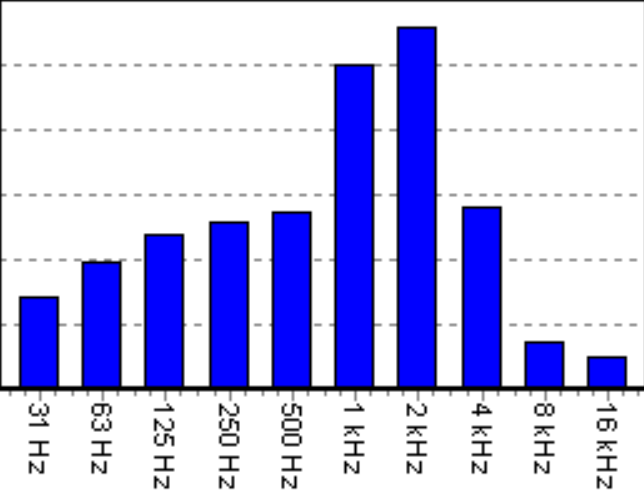
\includegraphics[width=0.8\linewidth]{fig/octave_band.PNG}
	\end{subfigure}
	\begin{subfigure}[b]{0.49\textwidth}
		\centering
		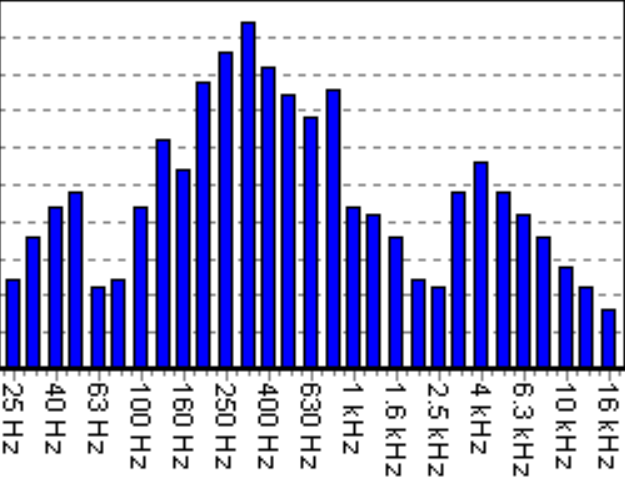
\includegraphics[width=0.8\linewidth]{fig/one_third_octave_band.PNG}
	\end{subfigure}
	\caption{Example octave band and 1/3-octave band spectra. Left: octave band spectrum. Right: 1/3-octave band spectrum. \cite{octave_band} }
	\label{fig:octave_band_filters}
\end{figure}

\noindent A widely used fractional octave band in the acoustic measurement is the 1/3-octave band, which is obtained by splitting each of the octave bands into three parts. Example sound spectra given in octave bands and 1/3-octave bands are shown in \cref{fig:octave_band_filters}. It can be seen that the spectrum in 1/3-octave bands contains more frequency bands than that of the octave band, allowing a more detailed analysis of the frequency content of the noise. Other common narrower fractional octave bands are for example 1/6-octave, 1/12-octave and 1/24-octave bands.

\newpage
\subsection{Frequency weighting}

\begin{figure}[H]
	\centering
	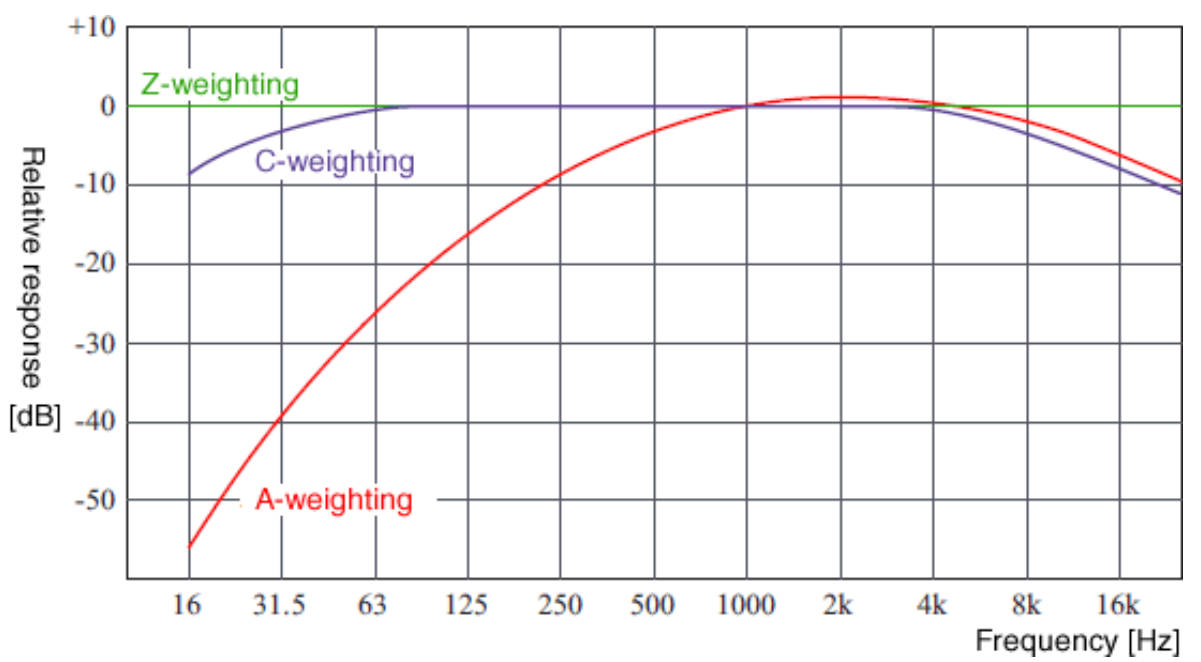
\includegraphics[width=0.8\textwidth]{fig/frequency_weighting.png}
	\caption{Frequency weighting (A, C and Z) \cite{Frquency_weighting}.}
	\label{fig:weighting}
\end{figure}

The human audible system does not respond equally to sound frequencies. It is more sensitive to frequencies between \SI{500}{\hertz} and \SI{8000}{\hertz} and less sensitive to lower-pitch and higher-pitch noises \cite{weighting_filters}. To match this frequency-dependent perception of sound loudness of the human ear, so-called frequency weighting filters have been defined, which can be seen as correction functions of the measured sound levels. However, the frequency response of the ear also depends on sound pressure level, at lower levels the effect is more pronounced than at higher levels \cite{heutschi_lecture_2016}. Therefore, several weighting filters have been defined. The most commonly used weighting functions are A-weighting and C-weighting, which are designed for low and high sound levels, respectively. If no weighting filter is applied to the measurement, it is also called Z-weighting. The response functions of the A, C and Z-weighting filters are shown in \cref{fig:weighting}.

In the ambient noise measurement, the most frequently used weighting is A-weighting. It can be calculated by the weighting function \cite{IEC61672}
\begin{equation}
	 R_A(f) = {12194^2 f^4 \over \left(f^2 + 20.6^2\right)\ \sqrt{\left(f^2 + 107.7^2\right)\left(f^2 + 737.9^2\right)}\ \left(f^2 + 12194^2\right)}\,,
\end{equation}
with $f$ being the frequency in \SI{}{\hertz}, the amplitude response of A-filter results in
\begin{equation}
	\text{A-weighting}(f) = 20\log_{10}\left(R_A(f)\right) - 20\log_{10}\left(R_A(1000)\right) \,. \label{eq:a_weighting}
\end{equation}
The second term in \cref{eq:a_weighting} is to ensure that the amplitude of the weighting function is normalized to \SI{0}{\decibel} at \SI{1000}{\hertz}, which can also be seen in \cref{fig:weighting}. Sound level measurements with A-weighting filter applied are expressed as dBA, or dB(A).

\newpage
\section{X-Wagen metro train}
\label{section:ubx_geometry}

In this thesis, the finite element modeling approach of underfloor noise prediction is applied to the X-Wagen metro from Siemens Mobility. A brief overview of the metro train is presented in the following section in order to provide a better insight into the modeled vehicle.

\begin{figure}[H]
	\centering
	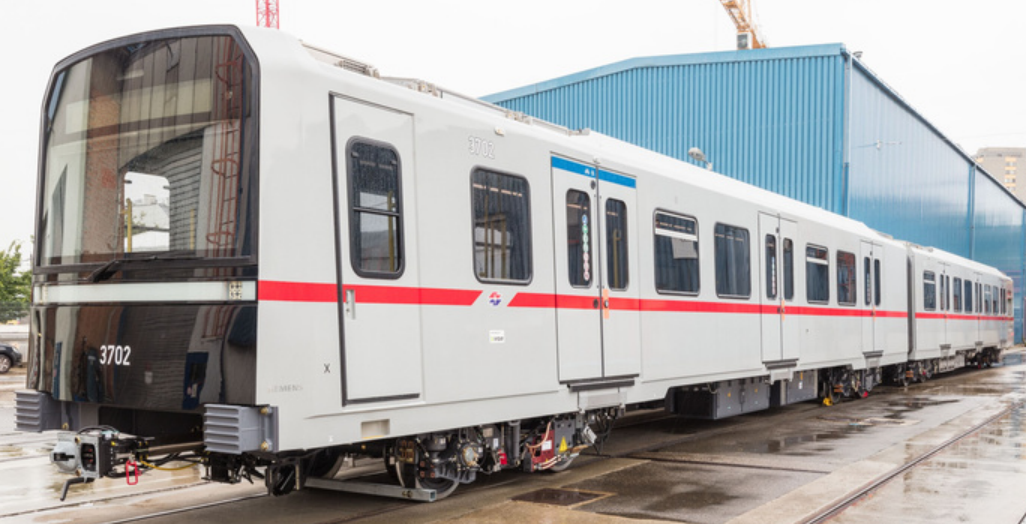
\includegraphics[width=0.8\textwidth]{fig/ubx_wiener_linien.PNG}
	\caption{The first X-Wagen metro train at Siemens Mobility plant Leberstraße \cite{foto_ubx}.}
	\label{fig:ubx_foto}
\end{figure}

The metro train Type X, also known as the X-Wagen, was developed by Siemens and is manufactured at the Siemens Mobility plant in Vienna. The third generation of the Vienna metro system aims to replace the old metro model Silberpfeil, which has been in operation since 1972. Siemens delivered the first X-Wagen (\cref{fig:ubx_foto}) in 2020, and the last vehicle is scheduled for delivery at the end of 2030.

\begin{figure}[H]
	\centering
	\begin{subfigure}[b]{\textwidth}
		\centering
		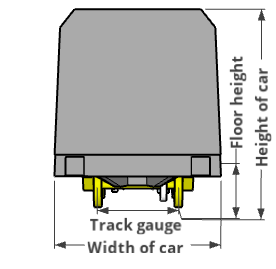
\includegraphics{fig/UBX_front_view_with_label_smaller.PNG}
		\caption{Front view}
	\end{subfigure}

	\begin{subfigure}[b]{\textwidth}
		\centering
		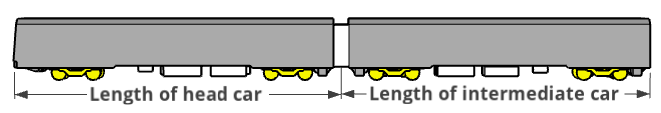
\includegraphics{fig/UBX_sketchup_model_side_view_with_label_2.PNG}
		\caption{Side view}
		\label{fig:ubx_model_sideview}
	\end{subfigure}
	
	\caption{Simplified 3D model of the X-Wagen in its basic configuration.}
	\label{fig:ubx_sketup_model}
\end{figure}

The basic configuration of the train, as shown in \cref{fig:ubx_foto} and \cref{fig:ubx_model_sideview}, consists of two metro cars, a non-motorized head car where the driver's cab is located, and a motorized intermediate car. One section of the metro car is about \SI{2.85}{\meter} in width and \SI{3.6}{\meter} in height and has a length of \SI{19.1}{\meter} for the head car and \SI{18.3}{\meter} for the intermediate car, respectively. The train has a standard track gauge of \SI{1.425}{\meter}, and the car floor is about \SI{0.95}{\meter} over top of the rail. In the operating configuration, the metro train is made up of 6 sections consisting of 2 head cars and 4 intermediate cars with a length of over \SI{110}{\meter}.

\begin{figure}[H]
	\centering
	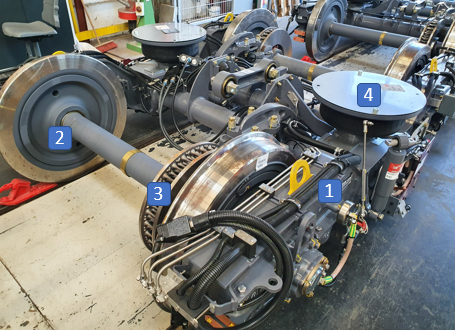
\includegraphics{fig/running_bogie_with_labels.PNG}
	\caption{A non-driven bogie from the head car. The main components are numbered as follows; (1) bogie frame, (2) wheel and axle, (3) brake disc, (4) air suspension.}
	\label{fig:bogie_foto}
\end{figure}

The main components in the train underfloor are the bogies and other supporting units like air compressors, electrical transformers, etc.
Each metro car is equipped with two bogies. While the bogies at the front car are non-driven, the intermediate car bogies are driven by traction motors. A non-driven bogie from the front car is shown in \cref{fig:bogie_foto} with the main components numbered. These are the bogie frame with a length of about \SI{3}{\meter}, the wheels with \SI{0.85}{\meter} diameter, and a distance of \SI{2}{\meter} to each other, the axles, and the air suspensions. Each axle is equipped with one brake disk and one brake caliper unit, and the brake components of both axles are arranged in an anti-symmetric order.

\begin{figure}[H]
	\centering
	\begin{subfigure}[b]{0.48\textwidth}
		\centering
		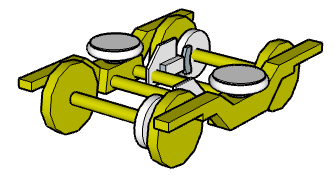
\includegraphics{fig/running_bogie_sketchup.PNG}
		\caption{Perspective view}
	\end{subfigure}
	\begin{subfigure}[b]{0.48\textwidth}
		\centering
		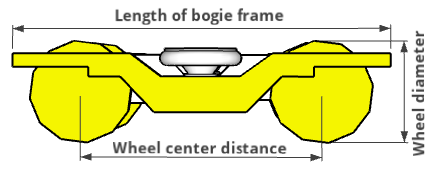
\includegraphics[width=\linewidth]{fig/running_bogie_sideview_with_labels.PNG}
		\caption{Side view}
		\label{fig:bogie_side_view}
	\end{subfigure}
	\label{fig:bogie_3d_model}
	\caption{Simplified 3D model of the non-driven bogie containing the main components as described in \cref{fig:bogie_foto}.}
\end{figure}

A simplified 3D model of the non-driven bogie containing the mentioned main components is shown in \cref{fig:bogie_3d_model}. One can see that the brake components introduce asymmetry into the bogie geometry. If they are disregarded, the symmetry of the bogie can be exploited, and the full model can be represented by a one-fourth model, which is used in the latter finite element modeling in \cref{chap:FEM}.
% kein Absatz ....
Finally, the mentioned dimensions of the metro car and of the bogie components in this section are summarized in \cref{tab:vehicle_dimensions}.
\begin{table}[H]
	\caption{Dimensions of metro car and bogie as shown in \cref{fig:ubx_sketup_model} and \cref{fig:bogie_side_view}.}
	\centering
	\begin{tabular}{lc}
		\toprule
		Parameter                    	   &  Dimension (mm)    \\
		\midrule
		\textbf{Metro car} 				   & 		 \\
		Width of car                       & 2,850   \\
		Height of car  					   & 3,588   \\
		Length of head car  			   & 19,125  \\
		Length of intermediate car 		   & 18,250  \\
		Floor height above top of rail     & 948     \\
		Track gauge              		   & 1,435   \\
		\textbf{Bogie} 					   & 		 \\
		Length of bogie frame    		   & 3,076   \\
		Wheel center distance 			   & 2,000   \\ 
		Wheel diameter  				   & 850     \\ 
		\bottomrule
	\end{tabular}
	\label{tab:vehicle_dimensions}
\end{table}